\documentclass[runningheads]{llncs}
\usepackage[T1]{fontenc}
\usepackage{graphicx}
\usepackage{amsmath,amssymb}
\usepackage{hyperref}

\begin{document}

\title{MoiraiVaR: VaR-Aware Adaptation of Time-Series Foundation Models for Volatility Forecasting}
\titlerunning{\relax}

\author{Nguyen Thien Nhan\inst{1}\orcidID{0009-0003-2461-1359} \and
Tran Hung Vi\inst{1}\orcidID{0009-0009-8341-9678} \and
Nguyen Dinh Thuan\inst{1}\orcidID{0000-0002-7762-1505}}
\authorrunning{\relax}
\institute{$^{1}$\enspace Faculty of Information Systems, University of Information Technology,\\
Ho Chi Minh City, Vietnam\\
Corresponding author e-mail: \email{thuannd@uit.edu.vn}}

\maketitle

\begin{abstract}
While time-series foundation models (TSFMs) achieve state-of-the-art point accuracy through large-scale pretraining, their zero-shot representations do not inherently capture asymmetric financial tail risk. We propose \textit{MoiraiVaR}, a parameter-efficient fine-tuning (PEFT) framework that aligns pretrained TSFMs with volatility forecasting via a VaR-aware joint objective. By coupling a frozen Moirai-family backbone to a compact regression head, we optimize mean squared error alongside a Student-$t$ Value-at-Risk pinball loss. Furthermore, we address critical flaws in machine-learning volatility evaluation through a three-layer protocol: a Forecast Sanity Gate to filter models exhibiting degenerate representation learning (e.g., constant forecasts), and an average-of-distributions VaR metric to prevent evaluator-induced distribution leakage. Evaluating 1.3 million predictions across 26 configurations, we demonstrate that MoiraiVaR--Moirai-MoE occupies a non-dominated position on the accuracy--tail Pareto frontier. Multi-criteria decision making confirms that this architecture ranks first globally by both SAW and TOPSIS under balanced and risk-priority policies, offering a robust representation for financial risk management.

\keywords{MoiraiVaR \and time-series foundation model \and volatility forecasting \and Value-at-Risk \and Pareto frontier \and multi-criteria decision making}
\end{abstract}

\section{Introduction}
Recent advances in time-series foundation models (TSFMs) have demonstrated strong zero-shot transfer capabilities through large-scale pretraining on heterogeneous data \cite{ref7,ref8}. While TSFMs excel at minimizing mean squared error (MSE) for point forecasting, their learned representations do not inherently optimize for asymmetric tail-risk applications such as Value-at-Risk (VaR). Relying solely on standard scalar losses fails to guarantee the realistic amplitude scaling required for financial decision-making \cite{ref1}.

To align foundation models with financial risk objectives, we propose \textit{MoiraiVaR}, a parameter-efficient fine-tuning (PEFT) framework. MoiraiVaR couples a frozen pretrained Moirai representation to a multi-horizon regression head, trained using a joint point--tail objective that minimizes MSE alongside a Student-$t$ VaR pinball loss.

In addition to the architecture, this paper introduces a robust three-layer machine-learning evaluation methodology designed to prevent common benchmarking flaws in volatility forecasting:

\begin{enumerate}
\item \textbf{Forecast Sanity Gate.} Deep-learning models optimizing standard losses frequently converge to degenerate representations, outputting near-constant predictions that achieve deceptively low MSE by predicting the global mean \cite{ref2}. This gate explicitly filters such uninformative sequences.
\item \textbf{Multi-Distribution VaR Protocol.} Evaluating a Student-$t$-trained network under Student-$t$ assumptions risks rewarding the model simply because the evaluator's metric matches the training loss. We prevent this evaluator-induced distribution leakage by averaging tail calibration across Normal, Student-$t$ \cite{ref10}, and Filtered Historical Simulation (FHS) \cite{ref11} constructions, testing the model's out-of-distribution robustness.
\item \textbf{Accuracy--Risk Pareto Framework.} We evaluate the intrinsic trade-off between predictive point accuracy and tail-risk calibration using dual-policy multi-criteria decision making (MCDM).
\end{enumerate}

Evaluating 26 configurations across 1.3 million predictions, our headline result establishes that MoiraiVaR--Moirai-MoE is the only architecture ranked first globally by both Simple Additive Weighting (SAW) and TOPSIS under balanced and risk-priority policies. It occupies a non-dominated position on the accuracy--tail Pareto frontier, providing the most robust representation across heterogeneous tail distributions.

\section{MoiraiVaR}
Let $r_t$ denote the percentage log return at time $t$, and let $x_t = (r_{t-59}, \dots, r_t)$ be the 60-day return context. The target $y_{t,h}$ is the $h$-day realized standard deviation of daily log returns:
\begin{equation}
y_{t,h} = \sqrt{\frac{1}{h} \sum_{k=1}^{h} r_{t+k}^2}.
\end{equation}

A frozen pretrained Moirai-family encoder processes the return context into a sequence of representations. Temporal mean pooling yields a fixed-size feature vector $h_t$, which feeds a two-layer multilayer perceptron to produce volatility forecasts $\hat{\sigma}_{t,h}$ for horizons $\mathcal{H} = \{1, 3, 5, 10, 21\}$. This parameter-efficient adaptation isolates whether a shared pretrained representation can be redirected toward volatility forecasting without full retraining.

For target $y_{t,h}$ and prediction $\hat{\sigma}_{t,h}$, the multi-horizon accuracy term is
\begin{equation}
\mathcal{L}_{\text{vol}} = \frac{1}{|\mathcal{B}|\,|\mathcal{H}|} \sum_{t\in\mathcal{B}} \sum_{h\in\mathcal{H}} (\hat{\sigma}_{t,h} - y_{t,h})^2.
\end{equation}

\begin{figure}[t]
\centering

\includegraphics[width=\textwidth]{fig_moirai_var_architecture.png}
\caption{MoiraiVaR couples a frozen Moirai-family backbone to a volatility head. Training combines multi-horizon MSE with a Student-$t$ VaR pinball loss.}
\label{fig1}
\end{figure}

The risk-aware penalty uses the one-step prediction and the 1\% lower Student-$t$ quantile:
\begin{equation}
v_{t,0.01} = \hat{\sigma}_{t,1} t_{0.01,\nu}.
\end{equation}

With $u_t = r_{t+1} - v_{t,0.01}$, the pinball loss \cite{ref9} is
\begin{equation}
\mathcal{L}_{\text{VaR}} = \frac{1}{|\mathcal{B}|} \sum_{t\in\mathcal{B}} \left(0.01 - \mathbf{1}\{u_t < 0\}\right) u_t.
\end{equation}

The joint objective is
\begin{equation}
\mathcal{L} = \mathcal{L}_{\text{vol}} + \lambda_{\text{VaR}} \mathcal{L}_{\text{VaR}}, \quad \lambda_{\text{VaR}} = 0.2.
\end{equation}

The degrees of freedom $\nu$ are estimated from the training-return excess kurtosis to adapt the tail term dynamically to market-level data. During parameter-efficient fine-tuning, only the downstream regression head is trained using AdamW (learning rate $10^{-3}$, weight decay $10^{-4}$), gradient clipping at 1.0, dropout of 0.2, and early stopping with a patience of seven epochs.

\section{Accuracy--Risk Evaluation Framework}
Our three-layer evaluation protocol ensures that rankings are dynamically informative and robust against distribution leakage.

\subsection{Layer 1: Multi-Distribution VaR Construction}
To decouple evaluation from the Student-$t$ training penalty, three VaR constructions are backtested independently via Kupiec and Christoffersen tests \cite{ref12,ref13}. The risk criteria entering the decision matrix cover Normal, conditional Student-$t$ \cite{ref10}, and filtered historical simulation (FHS) \cite{ref11}. They are the equally weighted averages of method-level pass rates $\text{PR}_\alpha$ and absolute violation errors $E_\alpha$ for $\alpha \in \{0.01, 0.05\}$. This design prevents models from appearing superior merely by matching the evaluator's distributional assumptions.

\subsection{Layer 2: Forecast Sanity Gate and Decision Matrix}
Deep-learning models can suffer from degenerate representation learning, where a near-constant sequence minimizes MSE by predicting the global mean. Such degenerate models can pass VaR backtests coincidentally without actually tracking volatility dynamics. To exclude these trivial local optima before ranking, a Forecast Sanity Gate requires all model outputs to exhibit at least 10\% of the realized target's variability ($s_{\hat{y}}/s_y \ge 0.1$) and an average tracking correlation $\bar{\rho} > 0$.

The remaining valid configurations are assessed on nine criteria grouped into two blocks:
\begin{itemize}
\item \textbf{Accuracy block (minimized):} MSE, MAE, QLIKE, amplitude error $e_\sigma = |s_{\hat{y}}/s_y - 1|$, and tracking-correlation error $e_\rho = 1 - \max\{\rho(y, \hat{y}), 0\}$.
\item \textbf{Risk block (maximized or minimized):} averaged VaR 1\%/5\% pass rates (PR; maximize) and violation errors ($E$; minimize).
\end{itemize}

\subsection{Layer 3: Pareto Non-Dominance and MCDM}
Configurations are first evaluated for Pareto non-dominance to explicitly map the accuracy--tail trade-off. We then apply two aggregation methods: SAW \cite{ref14} and TOPSIS \cite{ref15,ref16}. To ensure robust conclusions, a model is declared the winner only if it ranks first by both methods under both a \textit{balanced policy} (50\% Accuracy, 50\% Risk) and a \textit{risk-priority policy} (30\% Accuracy, 70\% Risk). Sensitivity checks varying the block weights and raising the tracking-correlation threshold confirm the stability of the final ranking.

\section{Experimental Study}

\subsection{Data and Competitors}
The source contains 1,322,330 daily prediction rows covering VN-Index, VN30, KOSPI, Nikkei 225, DAX 40, Euronext 100, IBEX 35, SMI, and S\&P 500 at horizons $\{1, 3, 5, 10, 21\}$. The 26 configurations form 1,170 configuration--market--horizon blocks. Competitors include four GARCH-family models (including FI-GARCH \cite{ref3}); twelve Transformer configurations based on Reformer, Informer, and Autoformer \cite{ref4,ref5,ref6}; Moirai, Moirai 2, and Moirai-MoE; their three VaR-aware adaptations; and four GARCH-/Wavelet--Autoformer hybrids. Five configurations fail the Sanity Gate and are excluded from MCDM ranking. Tier 1 denotes large foundation models, Tier 2 denotes parameter-efficient adaptations, and Tier 3 denotes unadapted baseline architectures.

\subsection{Implementation Details}
The dataset is split chronologically into training (70\%), validation (10\%), and testing (20\%) sets per market without look-ahead overlap. The primary experiment evaluates head-only adaptation at $\lambda_{\text{VaR}} = 0.2$, leaving the foundation backbone frozen. Omnibus Friedman tests across the 45 market--horizon blocks confirm statistically significant differences in point accuracy among configurations ($p < 10^{-150}$). SAW and TOPSIS then aggregate these heterogeneous performances into a policy-aware composite score.

\subsection{Main Rankings and Pareto Compromise}
Figure \ref{fig2} illustrates the accuracy--tail trade-off for the representative configurations. Moirai 2 anchors the accuracy extreme (lowest MSE), while GJR--GARCH anchors the pass-rate extreme (highest PR). MoiraiVaR--Moirai-MoE occupies a non-dominated interior position on this Pareto frontier: no evaluated configuration attains both lower point loss and higher averaged VaR pass rate.

\begin{table}[h]
\centering
\caption{MCDM ranks for the top five eligible configurations out of 21. Models are ordered by their balanced-policy SAW performance.}\label{tab1}
\begin{tabular}{lcccc}
\hline
& \multicolumn{2}{c}{50:50 policy} & \multicolumn{2}{c}{30:70 policy} \\
\cline{2-3} \cline{4-5}
Configuration & SAW rank & TOPSIS rank & SAW rank & TOPSIS rank \\
\hline
MoiraiVaR--Moirai-MoE & \textbf{1} & \textbf{1} & \textbf{1} & \textbf{1} \\
Moirai 2 & 2 & 4 & 3 & 9 \\
MoiraiVaR--Moirai 2 & 3 & 2 & 6 & 6 \\
Moirai-MoE & 4 & 3 & 5 & 7 \\
Moirai & 5 & 6 & 4 & 8 \\
\hline
\end{tabular}
\end{table}

Table \ref{tab1} reports the top five eligible configurations. Under 50:50, MoiraiVaR--Moirai-MoE obtains SAW 0.8426 and TOPSIS 0.8401, ranking first by both methods. Under 30:70, it remains first. MCDM therefore shows that this Pareto compromise point is the preferred choice under both a balanced and a risk-priority preference specification.

SAW and TOPSIS remain closely aligned: Spearman rank correlation is 0.981 ($p = 6.84 \times 10^{-15}$) under 50:50 and 0.877 ($p = 1.87 \times 10^{-7}$) under 30:70. The winner is therefore unchanged even though several lower-ranked candidates move substantially when risk receives more weight.

The winner is a compromise rather than a metric-wise dominator. Table \ref{tab2} compares it with the strongest pure-accuracy and pure-pass-rate alternatives. Moirai 2 has the lowest MSE, MAE, and QLIKE, and the highest tracking correlation. GJR--GARCH has the highest 1\% and 5\% VaR pass rates. MoiraiVaR--Moirai-MoE remains near the top of the accuracy criteria while improving the 5\% pass rate relative to the unadapted Moirai-MoE from 0.304 to 0.393. Its 1\% and 5\% absolute violation errors also decline from 0.00829 to 0.00786 and from 0.01036 to 0.01008.

\begin{table}[h]
\centering
\caption{Raw aggregate metrics for representative configurations. Lower is better for losses and violation error; higher is better for correlation and pass rate. Bold entries identify the best value in each column.}\label{tab2}
\resizebox{\textwidth}{!}{
\begin{tabular}{lcccccccc}
\hline
Configuration & MSE & MAE & QLIKE & $\rho$ & $\text{PR}_{.01}$ & $E_{.01}$ & $\text{PR}_{.05}$ & $E_{.05}$ \\
\hline
MoiraiVaR--Moirai-MoE & 0.02526 & 0.10149 & 0.00932 & 0.899 & 0.304 & 0.00786 & 0.393 & \textbf{0.01008} \\
Moirai-MoE & 0.02476 & 0.09756 & 0.00913 & 0.898 & 0.296 & 0.00829 & 0.304 & 0.01036 \\
Moirai 2 & \textbf{0.02275} & \textbf{0.09062} & \textbf{0.00912} & \textbf{0.916} & 0.296 & 0.00781 & 0.289 & 0.01016 \\
GJR--GARCH & 0.19112 & 0.29196 & 0.05141 & 0.444 & \textbf{0.348} & \textbf{0.00623} & \textbf{0.526} & 0.01114 \\
\hline
\end{tabular}
}
\end{table}

The SAW score decomposition makes the balance explicit. Under 50:50, MoiraiVaR--Moirai-MoE receives 0.4907 from the forecast/dynamics block and 0.3518 from the VaR block. Under 30:70, the components become 0.2944 and 0.4926. GJR--GARCH obtains the larger 30:70 risk component (0.6241), but its accuracy component is only 0.1362. MoiraiVaR thus avoids the severe accuracy sacrifice associated with optimizing pass rates in isolation.

\begin{figure}[t]
\centering
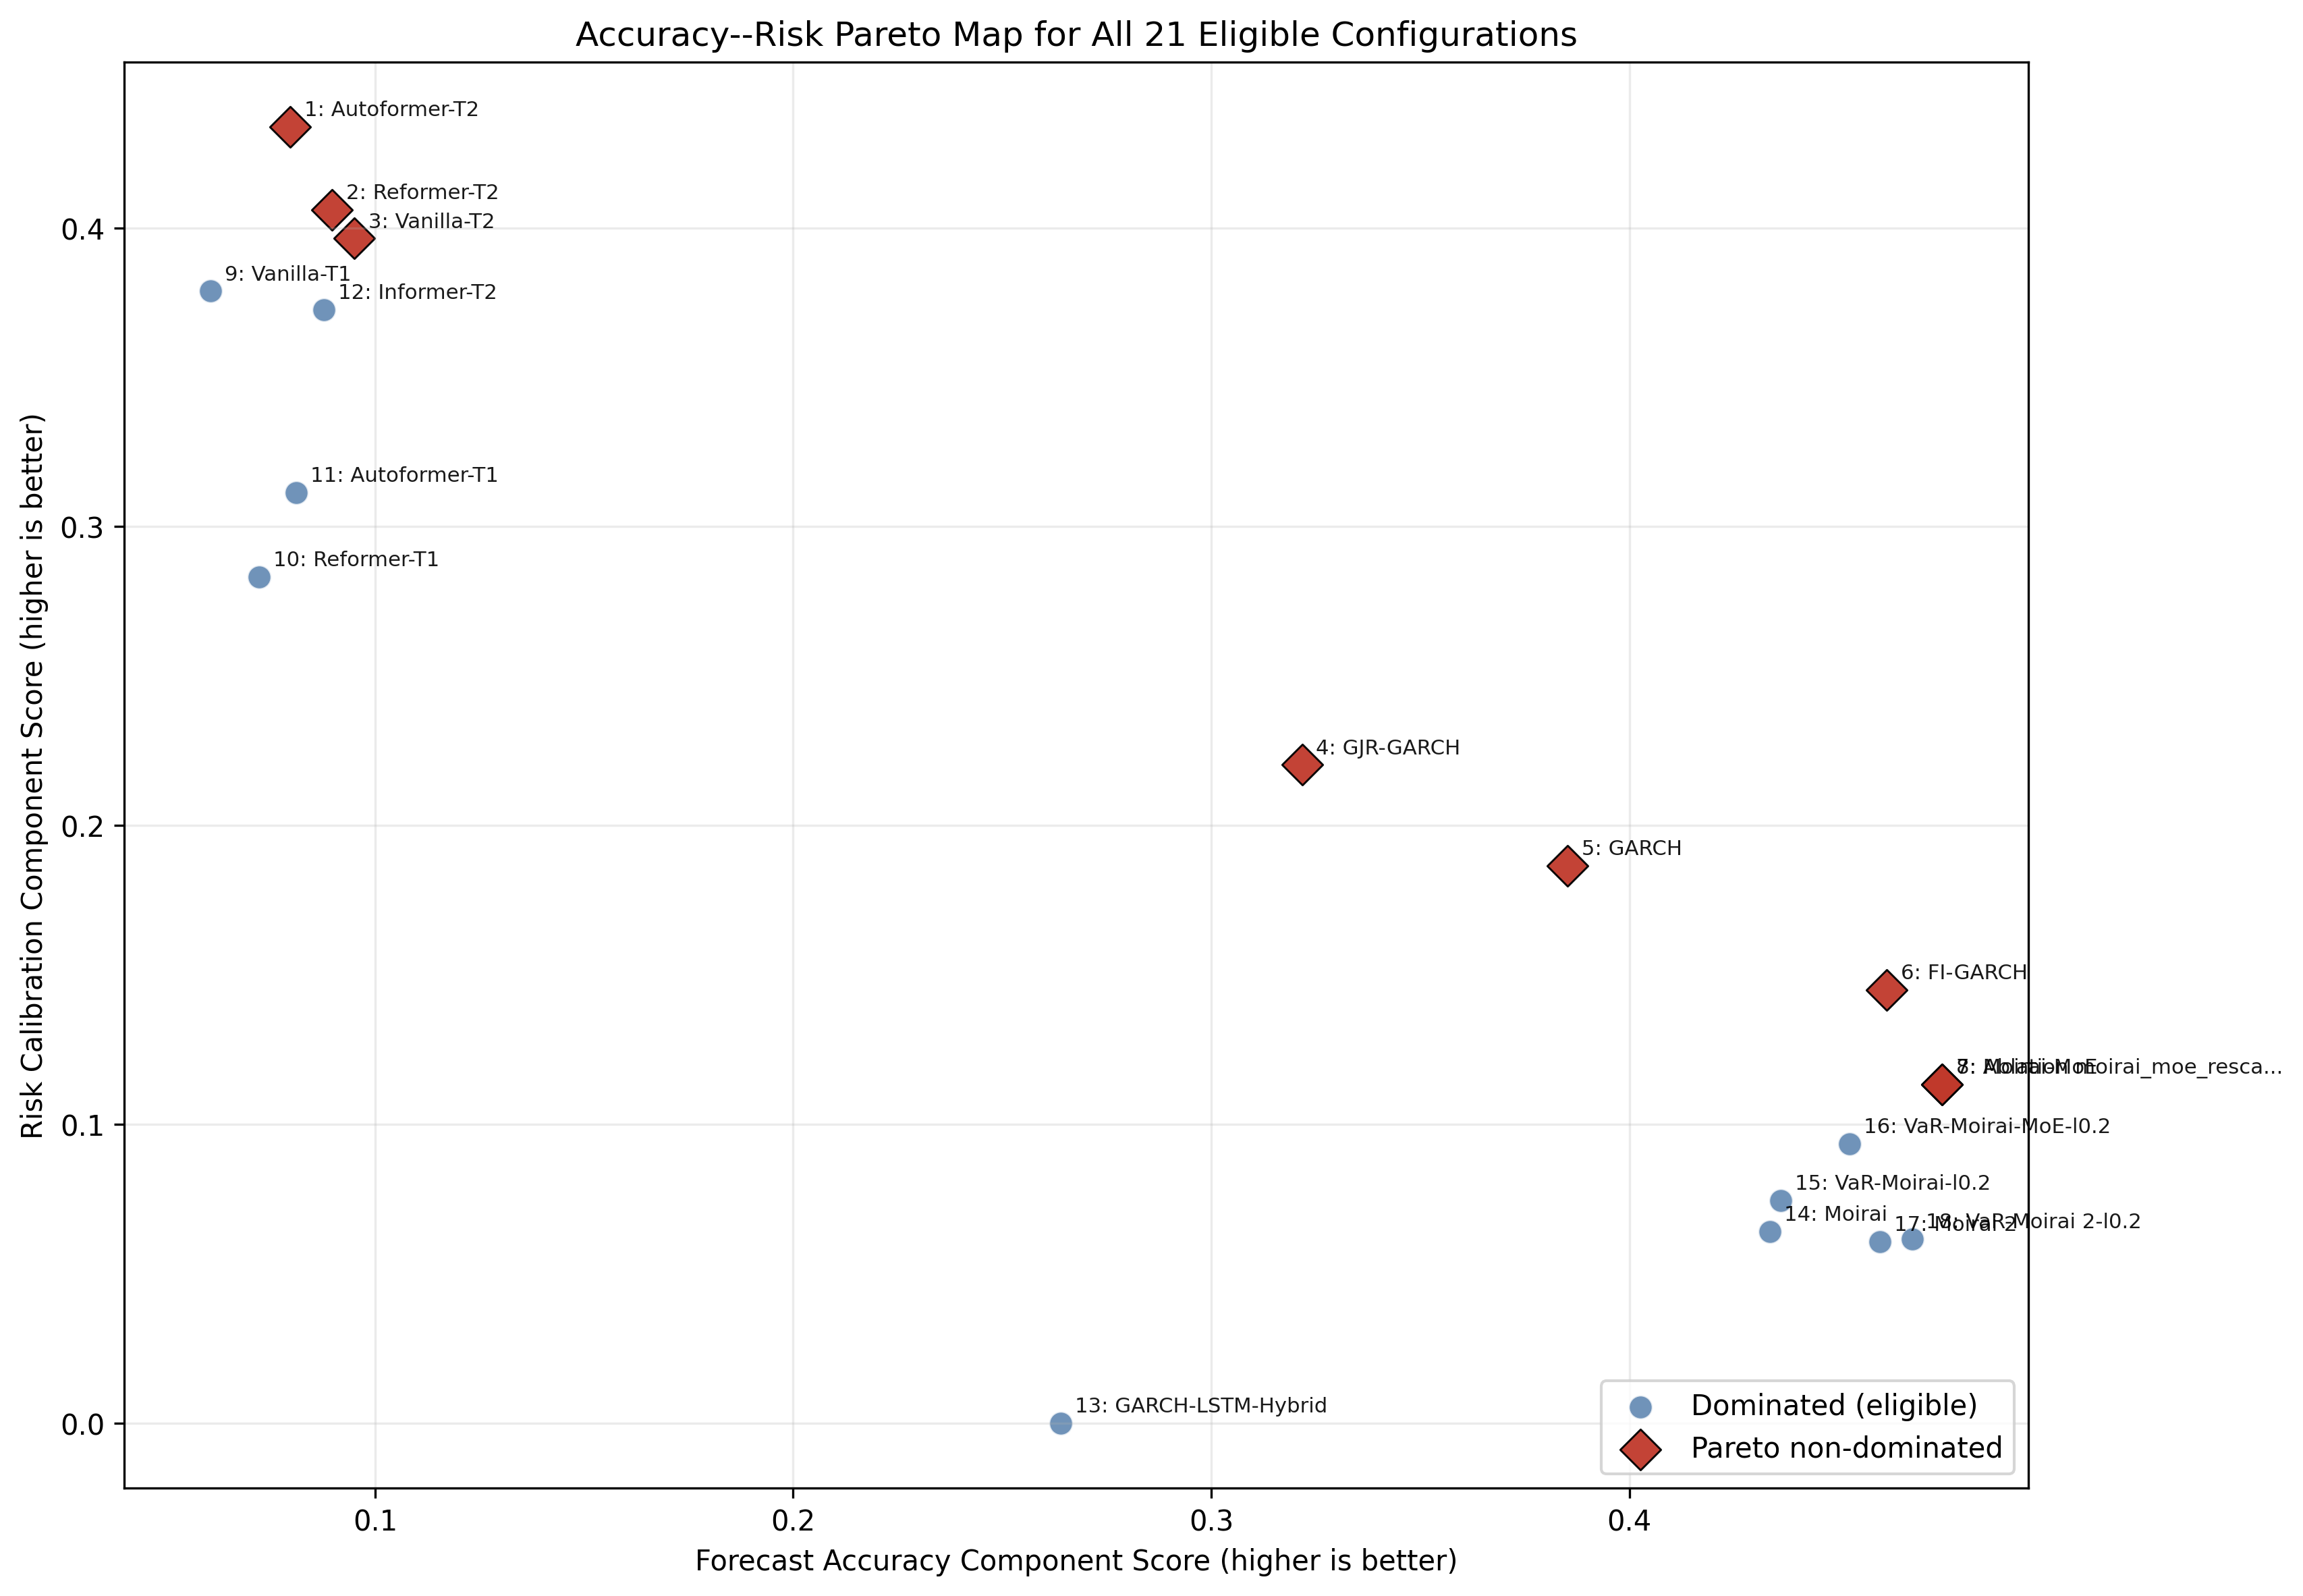
\includegraphics[width=\textwidth]{fig_accuracy_risk_pareto.png}
\caption{Accuracy--Risk Pareto frontier for representative configurations. Moirai 2 anchors the point-accuracy extreme (lowest MSE), while GJR--GARCH anchors the VaR calibration extreme (highest 5\% pass rate). MoiraiVaR--Moirai-MoE occupies a non-dominated interior compromise position. Configurations strictly inside the curve are Pareto-dominated.}
\label{fig2}
\end{figure}

\subsection{Robustness of the Balance Claim}
MoiraiVaR--Moirai-MoE remains first by both methods at accuracy weights 0.30, 0.40, 0.50, 0.60, and 0.70. It also remains first when the minimum tracking-correlation threshold increases from 0 to 0.05 and 0.10, which reduces the eligible set from 21 to 16 and 13 configurations. These checks show that its consensus rank is not produced by one weight split or by weakly dynamic competitors near the Gate boundary.

Tail-model sensitivity is stronger. Under Normal-only criteria, FI-GARCH is the consensus winner; under Student-$t$-only criteria, GARCH--Autoformer Tier 2 ranks first; and under FHS-only risk priority, GJR--GARCH ranks first. For MoiraiVaR--Moirai-MoE itself, the 1\% pass rates are 0.556, 0.156, and 0.200 for FHS, Normal, and Student-$t$. At 5\%, they are 0.511, 0.578, and 0.089. The averaged primary analysis rewards a configuration that performs comparatively well across these conflicting constructions, but it does not imply invariance to the choice of tail model.

\section{Discussion and Limitations}
The main result supports a specific form of risk-aware transfer. Rather than finding a universally superior forecast, the VaR-aware objective shifts the model along the Pareto frontier, trading modest accuracy gaps (a 2.0\% MSE increase relative to Moirai-MoE) for improved average VaR calibration. Reporting these positions explicitly prevents a single composite rank from obscuring the raw trade-off.

Several limitations bound these conclusions:
\begin{itemize}
\item \textbf{Low absolute pass rates.} The highest averaged 5\% pass rate remains below 60\%, indicating that no evaluated configuration achieves fully satisfactory practical VaR calibration.
\item \textbf{Rescaling baseline.} We did not ablate against a post-hoc scalar-tuned baseline $\hat{\sigma} \times c$; future work must verify whether the improvements stem from learned representations or simple scale inflation.
\item \textbf{Unscaled quantile thresholds.} The evaluation applies standard Student-$t$ quantiles without the $\sqrt{\nu/(\nu - 2)}$ variance scale factor, yielding conservative thresholds that depress pass rates for heavy-tailed predictions.
\item \textbf{Temporal leakage risk.} The dataset lacks strict purging/embargo periods between the chronological splits, potentially leaking forward information.
\item \textbf{Missing baselines.} Econometric baselines such as HAR-RV and EWMA/RiskMetrics were not included.
\end{itemize}

\section{Conclusion}
MoiraiVaR connects a pretrained time-series foundation model to financial tail-risk requirements through a VaR-aware joint objective. Extensive multi-distribution evaluation confirms that MoiraiVaR--Moirai-MoE provides the most robust, distribution-averaged compromise for financial risk management, ranking first by both SAW and TOPSIS across balanced and risk-priority policies.

\subsubsection{AI Disclosure.} Generative AI assisted with manuscript organization and language editing; the authors verified the research design, results, claims, and references.

\subsubsection{Acknowledgements.}This research was supported by The VNUHCM-University of Information Technology's Scientific Research Support Fund.

\begin{thebibliography}{8}

\bibitem{ref1}
Bollerslev, T.: Generalized autoregressive conditional heteroskedasticity. J. Econometrics \textbf{31}(3), 307--327 (1986).

\bibitem{ref2}
Patton, A.J.: Volatility forecast comparison using imperfect volatility proxies. J. Econometrics \textbf{160}(1), 246--256 (2011).

\bibitem{ref3}
Baillie, R.T., Bollerslev, T., Mikkelsen, H.O.: Fractionally integrated generalized autoregressive conditional heteroskedasticity. J. Econometrics \textbf{74}(1), 3--30 (1996).

\bibitem{ref4}
Kitaev, N., Kaiser, L., Levskaya, A.: Reformer: The efficient Transformer. In: ICLR (2020).

\bibitem{ref5}
Zhou, H., et al.: Informer: Beyond efficient Transformer for long sequence time-series forecasting. In: AAAI, vol. 35(12), pp. 11106--11115 (2021).

\bibitem{ref6}
Wu, H., Xu, J., Wang, J., Long, M.: Autoformer: Decomposition Transformers with auto-correlation for long-term series forecasting. In: NeurIPS, vol. 34, pp. 22419--22430 (2021).

\bibitem{ref7}
Woo, G., Liu, C., Kumar, A., Xiong, C., Savarese, S., Sahoo, D.: Unified training of universal time series forecasting Transformers. In: ICML, PMLR 235, pp. 53140--53164 (2024).

\bibitem{ref8}
Liu, X., Liu, J., Woo, G., Aksu, T., Liang, Y., Zimmermann, R., Liu, C., Li, J., Savarese, S., Xiong, C., Sahoo, D.: Moirai-MoE: Empowering time series foundation models with sparse mixture of experts. In: ICML, PMLR 267, pp. 38940--38962 (2025).

\bibitem{ref9}
Koenker, R., Bassett, G., Jr.: Regression quantiles. Econometrica \textbf{46}(1), 33--50 (1978).

\bibitem{ref10}
Bollerslev, T.: A conditionally heteroskedastic time series model for speculative prices and rates of return. Rev. Econ. Stat. \textbf{69}(3), 542--547 (1987).

\bibitem{ref11}
Barone-Adesi, G., Giannopoulos, K., Vosper, L.: VaR without correlations for portfolios of derivative securities. J. Futures Mark. \textbf{19}(5), 583--602 (1999).

\bibitem{ref12}
Kupiec, P.H.: Techniques for verifying the accuracy of risk measurement models. J. Derivatives \textbf{3}(2), 73--84 (1995).

\bibitem{ref13}
Christoffersen, P.F.: Evaluating interval forecasts. Int. Econ. Rev. \textbf{39}(4), 841--862 (1998).

\bibitem{ref14}
Triantaphyllou, E.: Multi-Criteria Decision Making Methods: A Comparative Study. Springer, New York (2000).

\bibitem{ref15}
Hwang, C.L., Yoon, K.: Multiple Attribute Decision Making: Methods and Applications. Springer, Berlin, Heidelberg (1981).

\bibitem{ref16}
Behzadian, M., Otaghsara, S.K., Yazdani, M., Ignatius, J.: A state-of-the-art survey of TOPSIS applications. Expert Syst. Appl. \textbf{39}(17), 13051--13069 (2012).

\end{thebibliography}
\end{document}
